\chapter{System considerations}
\section{Platform}
We have worked with several different platforms throughout the courses in our education. A valid choice for platform would be the PSoC 3(5) that we had already worked on. We had been told from other students taking this course that the PSoC was not ideal for sound processing and that the blackfin platform had built in features for this. We had no idea how to use the blackfin so it was a great opportunity to learn to use another platform. 
\subsection{PSoC}
Speed\\
I/O\\
ADC/DMA\\
Memory\\
\subsection{Blackfin}
\textbf{Speed:}\\
The blackfin processor runs at 600MHz. For every clock it can do two operations (multiplication and/or addition). This effectively means that we can do 1200 million operations per second, if we use the processor 100\% of the time.\\
\textbf{I/O}\\
\fxnote{Jeg skal skrives}\\
\textbf{ADC \& Audiocodec:}\\
The blackfin has a built-in audiocodec consisting of 4 ADCs and 6 DACs with a resolution of 24 bits. It has a signal to noise ratio of 105dB\footnote{http://www.analog.com/en/audiovideo-products/audio-codecs/ad1836/products/product.html}. There is an example project in the VisualDSP++ environment explaining how to utilize this codec.\\
\textbf{Memory:}\\
Since we do not use much memory we use the L1 cache in the BF533. It is according to the datasheet 32Kbytes big. Since we work with the datatype "short", which is 16 bits, we have enough space for 16K samples.\\
\begin{figure}[hbpt]
\centering
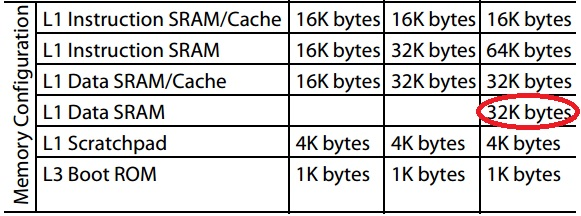
\includegraphics[width=0.5\textwidth]{billeder/memorytable}
\caption[Screen dump from datasheet]{Screen dump from datasheet\footnotemark}
\label{img:mem_table}
\end{figure}
\footnotetext{\url{http://www.analog.com/static/imported-files/data_sheets/ADSP-BF531_BF532_BF533.pdf}}
\subsection{DK8K}
We chose to ignore the DK8K platform as it does not have an Interactive Developer Environment(IDE). This would put a bigger workload on us but would not help us understand how to take advantage of Digital signal processing on embedded units.
\section{Fixed-/FloatingPoint}
\fxnote{Jeg skal skrives}
\section{Technology}
\subsection{Ultrasound}
The first method we discussed was ultrasound. But if we were to choose ultrasound we wouldnt have much data processing since we would just have a transmitter/reciever circuit which has an electrical interface. And wo wouldnt learn much about implementing digital signal processing. Peter also 

\subsection{Laser}
We didnt realy consider laser since we would rather try to play around with sound and measurements of sound. We also figured it would be a lot more complicated for this type of project.

\subsection{Audio}
We went along with hearable sound by suggestion from Peter. Hearable sound is easier to work with since, yes we can hear it, but it is easier to measure and produce. When we record sound we also get a lot of sample which we can process.

\section{Equipment}
\subsection{I/O}

\subsection{Ultrasonic sensor}
We had an ultrasonic sensor of the brand "Ping)))". This didnt really conflict with the concern about using ultrasound since it had a simple electrical interface, but it was not much about digital signal processing but more about timing so we didn't feel it was a good way to go.
\subsection{Speaker/Mic}